\begin{center}
\textsc{\Large Laboratorio 13}~\\
{\large Videojuegos, Físicas, Programación}~\\
\emph{Física en Videojuegos, Simulaciones y Ragdolls}
\end{center}

\section{Pre-Laboratorio}
\begin{itemize}
\item Investigar:
\begin{enumerate}
  \item Las tres leyes del movimiento de Newton.
  \item Cálculos en punto flotante en simulaciones físicas y errores.
  \item Determinismo y no-determinismo en simulaciones físicas.
\end{enumerate}
\item De algún juego que conozca analice.
\begin{enumerate}
  \item ¿En algún momento son utilizadas simulaciones físicas? 
  \item Si el juego posee simulaciones físicas ¿cual cree que sea el propósito de estas?
  \item En caso de no tener simulaciones físicas ¿considera algún caso donde el juego se pueda beneficiar de agregar simulaciones físicas?
\end{enumerate}
\item Investigar según su herramienta de trabajo como incorporar simulaciones físicas, rag-dolls, partículas y proyectiles tanto en 3D como en 2D. Recomendado practicar con ejemplos especialmente en 2D.
\end{itemize}

\section{Introducción}
Para agregar realismo, nuevas mecánicas o mayor calidad visual se introducen leyes físicas dentro del motor de juego, es mayormente usado en juegos tridimensionales \cite[p.~325]{jenkinscreatinggames}. Estas nuevos efectos se introducen en forma de simulaciones las cuales son aproximaciones de fenómenos reales utilizando valores discretos \cite{ian_gamephysics}. En el ambiente de un videojuegos una simulación completa y totalmente correcta podría causar complicaciones en las mecánicas de juego, progreso de la historia o hacer tediosas ciertas actividades.

\section{Simulaciones Físicas}
\setlength\intextsep{0pt}
\begin{wrapfigure}[8]{l}{0.4\linewidth}
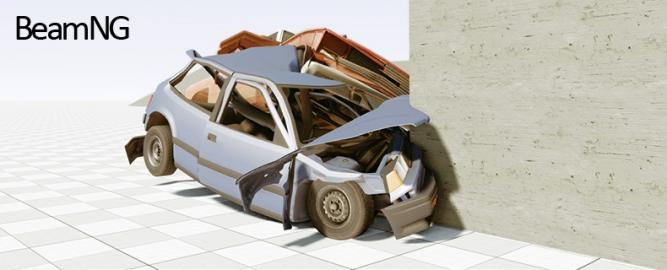
\includegraphics[width=\linewidth]{media/beamng_gamephysics.jpg}
\caption{BeamNG un videojuego simulador de vehiculos que utiliza \emph{soft-body physics}.}
\label{fig:beamng}
\end{wrapfigure}
Hay dos clases centrales de simulaciones físicas, simulaciones de cuerpos rígidos (\emph{rigid-body physics}) y simulaciones de cuerpos blandos (\emph{soft-body physics}). En una simulación de cuerpos rígidos los objetos se agrupan entre categorías basadas en como deberían interaccionar, las simulaciones de cuerpos rígidos son menos intensas en cuanto a perdida de \emph{performance}. Las simulaciones de cuerpos blandos consisten en simular secciones individuales de cada objeto de tal forma que este se comporte de manera realista, usualmente utilizadas para simular objetos deformables como ropa o materiales destructibles \cite{ian_gamephysics}.
\section{Físicas \emph{Ragdoll}}
\setlength\intextsep{0pt}
\begin{wrapfigure}[10]{r}{0.4\linewidth}
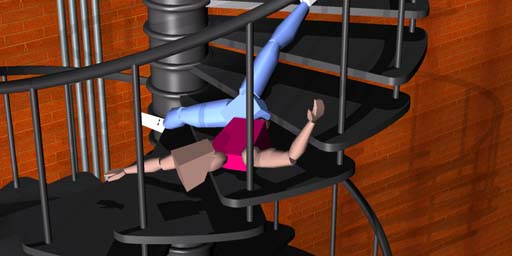
\includegraphics[width=\linewidth]{media/ragdoll.jpg}
\caption{Simulación de un personaje cayendo unas escalera, se utiliza un \emph{ragdoll}.}
\label{fig:ragdoll}
\end{wrapfigure}
Es una técnica de simulación que consiste en la animación procedimental de un personaje cuando este muere (u otro estado definido por el juego para causar \emph{ragdoll}, consiste en tratar a un objeto o personaje como una serie de objetos sólidos (huesos) conectados en distintos puntos formando un esqueleto. La simulación ocurre cuando el evento necesario para causar físicas \emph{ragdoll} sobre un objeto o personaje sucede, en los videojuegos esto pasa usualmente cuando el personaje muere \cite{eric_ragdoll}.

\section{Actividad}
Durante esta actividad se busca agregar físicas al juego para mejorar la inmersión y calidad visual del juego. Este laboratorio se enfocara en el uso de simulaciones físicas con el uso de rigid-bodies (cuerpos rígidos)
\begin{itemize}
\item Se debe hacer uso de rigid-bodies para varios objetos en escena.
\item Provocar un eventos al colisionar con un objeto rigid-body.
\item Asociar alguna acción al evento de colisión con un rigid-body, como reproducir un sonido o disminuir alguna propiedad asociada al jugador principal (como los puntos de vida, etc).
\end{itemize}
